\section{\method{}: Self-Distillation with Trajectory Intervention}
\label{sec:method}

Section~\ref{sec:analysis} shows that a teacher-preferred token can redirect student generation even when it does not repair the sampled response in place. Based on this observation, we propose \method{}, a simple branch--regenerate--distill algorithm that forces a teacher-selected token at a selected branch point, returns suffix generation to the student, and distills the resulting trajectory. We describe the algorithm in \S\ref{sec:algorithm}, motivate student-side regeneration in \S\ref{sec:method-student-generation}, and analyze the additional supervision created by regenerated trajectories in \S\ref{sec:method-collection-bottleneck}.


\begin{figure}[t]
  \centering
  \begin{subfigure}[t]{0.49\linewidth}
    \centering
    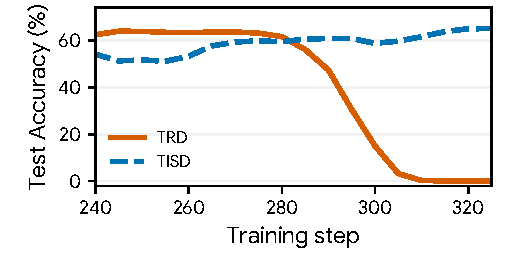
\includegraphics[width=\linewidth]{figures/trd_biology_validation.pdf}
    \caption{Avg@128 across training steps.}
    \label{fig:trd-biology-validation}
  \end{subfigure}
  \hfill
  \begin{subfigure}[t]{0.49\linewidth}
    \centering
    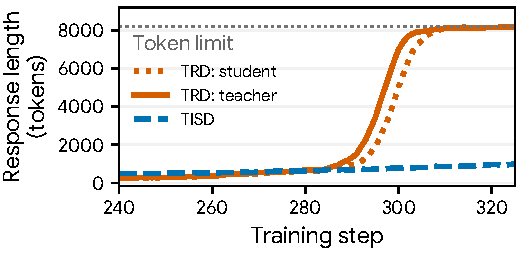
\includegraphics[width=\linewidth]{figures/trd_biology_response_length.pdf}
    \caption{Mean response length across training steps.}
    \label{fig:trd-biology-response-length}
  \end{subfigure}
  \captionsetup{skip=5pt}
  \caption{Training collapse of distillation on fully teacher-regenerated rollouts (TRD) on SciKnowEval L3 biology (Qwen3-8B).}
  \label{fig:trd-biology-collapse}
  \vspace{-0.2cm}
  
  
  
  
  
  
\end{figure}

\subsection{\method{} Algorithm}
\label{sec:algorithm}

\paragraph{Trajectory construction.}
Consider one collection iteration for prompt $x$, with student and self-teacher parameters $\theta$ and $\phi$ fixed during trajectory collection. Let $\pi_{\theta}(\cdot\mid x,y_{<t})$ denote the student distribution over vocabulary $\mathcal{V}$, and let $\pi_{\phi}(\cdot\mid x,y_{<t},c)$ denote the self-teacher distribution conditioned additionally on privileged context $c$. The behavior policy $\beta_{\theta}$ is the sampling policy induced by $\pi_{\theta}$ under the rollout decoding configuration, including temperature and truncation. We distinguish $\beta_{\theta}$ from the underlying model distributions used for branch selection and distillation.

First draw an initial response $y=(y_1,\ldots,y_T)\sim\beta_{\theta}(\cdot\mid x)$ with length $T$, obtain verifier reward $R(y)\in\{0,1\}$, and construct privileged context $c_y$. A successful response is retained unchanged, while a failed response is regenerated when the required privileged context is available. For an eligible failure, \method{} selects the peak-divergence position
\begin{equation}
\tstar
=
\operatorname*{argmax}_{1\leq t<T}
\mathcal D_t\!\left(
\pi_{\theta}(\cdot\mid x,y_{<t}),
\pi_{\phi}(\cdot\mid x,y_{<t},c_y)
\right).
\label{eq:repo-branch-position}
\end{equation}
\method{} then selects the teacher's most likely action at this prefix,
\begin{equation}
\hat y_{\tstar}
=
\operatorname*{argmax}_{a\in\mathcal{V}}
\pi_{\phi}(a\mid x,y_{<\tstar},c_y).
\label{eq:repo-branch-action}
\end{equation}
The teacher-preferred action may coincide with the original student token, $\hat y_{\tstar}=y_{\tstar}$; in this case, resampling the suffix can still expose additional contexts for teacher supervision. \method{} preserves the original prefix, forces $\hat y_{\tstar}$, and returns generation to the student:
\begin{equation}
\tilde y
=
\left(y_{<\tstar}, \; \hat y_{\tstar}, \; \widetilde y_{>\tstar}\right),
\qquad
\tilde y_{>\tstar}
\sim
\beta_{\theta}(\cdot\mid x,y_{<\tstar},\hat y_{\tstar}).
\label{eq:repo-conditional-law}
\end{equation}
The retained trajectory is $z=\tilde y$ for an eligible failed response and $z=y$ otherwise. Thus, the training data include original trajectories as well as regenerated trajectories whose outcomes may remain unsuccessful or become successful.


\vspace{-0.1cm}\paragraph{Distillation on the retained trajectory.}
For both unchanged and regenerated responses, \method{} minimizes teacher--student divergence along the retained trajectory using the privileged context $c_y$ associated with the original rollout and the SDPO objective~\citep{hubotter2026sdpo}:
\begin{equation}
\ell_{\mathrm{dist}}(z,c_y;\theta)
=
\frac{1}{|z|}
\sum_{t=1}^{|z|}
\mathcal D_t\!\left(
\pi_\theta(\cdot\mid x,z_{<t}),
\sg\!\left[
\pi_{\phi}(\cdot\mid x,z_{<t},c_y)
\right]
\right),
\label{eq:repo-per-trace-loss}
\end{equation}
where $\mathcal D_t$ is the divergence metric and $\sg[\cdot]$ denotes stop-gradient.


\subsection{Why Return Generation to the Student?}
\label{sec:method-student-generation}

\method{} returns suffix generation to the student to limit the mismatch between training trajectories and student generation at inference. TRD~\citep{jiang2026trajectory} revises the response using a privileged-context teacher, so the resulting suffix may follow actions and prefixes that the unconditioned student would be unlikely to generate on its own. In \method{}, the teacher determines only the branch action, while all subsequent tokens are sampled from the student's conditional behavior policy (Equation~\ref{eq:repo-conditional-law}). This exposes an alternative branch while keeping the continuation generated by the student itself.



\vspace{-0.1cm}\paragraph{Training instability of teacher regeneration.}
Figure~\ref{fig:trd-biology-collapse} shows a TRD run on SciKnowEval L3 biology with Qwen3-8B. From step 245 to 320, validation Avg@128 falls from 64.8\% to 0.0\%. Over the same interval, the mean student- and teacher-generated response lengths increase from 282 and 270 tokens to 8,192 and 8,167 tokens, respectively, approaching the generation limit. A validation response from this run also contains repetitive claims of alignment with a ``reference solution'' that is unavailable at inference (Appendix~\ref{app:trd-validation-example}). These results demonstrate the training instability of full-teacher regeneration and motivate returning suffix generation to the student in \method{}.

\subsection{\method{} Creates New Opportunities for Teacher Supervision}
\label{sec:method-collection-bottleneck}


\begin{figure}[t]
  \centering
  \begin{subfigure}[t]{0.722\linewidth}
    \centering
    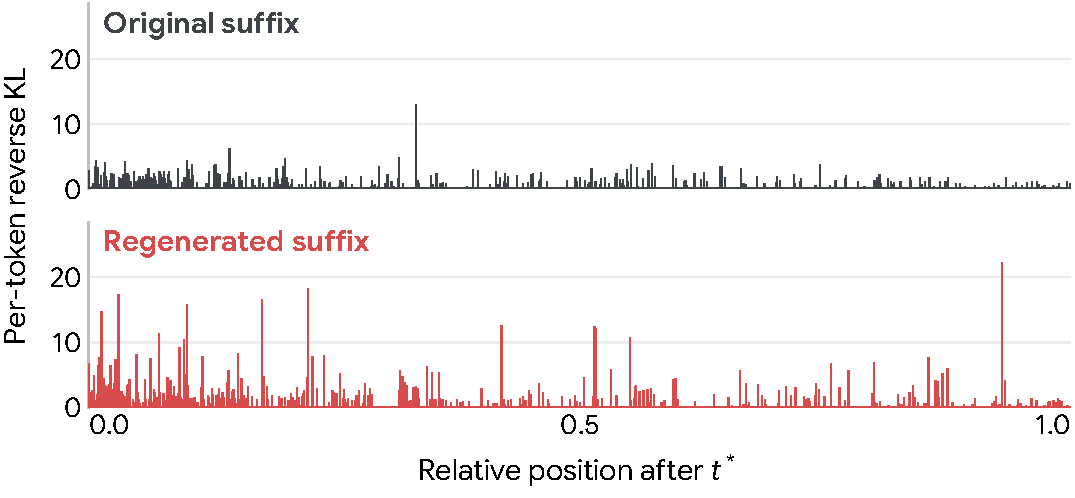
\includegraphics[width=\linewidth]{figures/fig_suffix/significant_illustration_token_kl.pdf}
    \caption{Aggregated token-level reverse KL profiles.}
    \label{fig:suffix-token-kl}
  \end{subfigure}
  \hfill
  \begin{subfigure}[t]{0.258\linewidth}
    \centering
    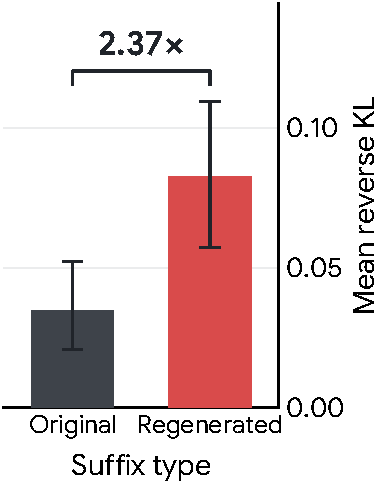
\includegraphics[width=\linewidth]{figures/fig_suffix/significant_illustration_mean_kl.pdf}
    \caption{Mean reverse KL.}
    \label{fig:suffix-mean-kl}
  \end{subfigure}
  \caption{Token-level KL-divergence from original and token-changed regenerated suffixes. Results aggregate failed rollouts from LiveCodeBench v6 of the base model (Qwen3-8B).}
  \label{fig:suffix-kl-comparison}
  \vspace{-8pt}
\end{figure}



In standard OPSD, supervising a teacher-preferred action at an observed prefix does not provide supervision at the successor prefixes induced by that action unless the student enters the corresponding branch during collection. This limitation is especially relevant when the student assigns low probability to the teacher-preferred action and therefore rarely visits the branch under on-policy sampling. \method{} instead forces the teacher-selected action, lets the student regenerate the suffix from the intervened prefix, and distills the resulting trajectory using Equation~\ref{eq:repo-per-trace-loss}. This makes teacher supervision available at the branch-induced successor prefixes within the same collection iteration.

Importantly, this benefit is not limited to early training. Even when the teacher targets on the original trajectories are well fitted, the student's predictions at intervention-induced prefixes need not be similarly aligned with the teacher (Appendix~\ref{app:conditional-advantage}, Proposition~\ref{prop:ident-ambiguity}). Thus, regenerated trajectories can introduce teacher supervision constraints that are absent from the original trajectories.









\vspace{-0.1cm}\paragraph{Regenerated suffixes expose additional teacher--student discrepancies.}
In the Qwen3-8B LiveCodeBench v6 diagnostic, regenerated suffixes after intervention have a mean token reverse KL that is $2.37\times$ that of their paired original suffixes (Figure~\ref{fig:suffix-kl-comparison}). This indicates that a single teacher-selected action can move the student into successor contexts with substantially larger teacher--student distribution disagreement, even though the continuation itself is generated by the student. These newly visited contexts provide additional targets for teacher supervision, whose downstream training effect is evaluated in Section~\ref{sec:experiments}.



































































































































































































































































































































































































































































































































































































































































































































































































































































































